\documentclass[10pt,a4paper]{article}

\usepackage[a4paper,top=16mm,bottom=17mm,left=18mm,right=18mm]{geometry}
\usepackage{fontspec}
\usepackage{microtype}
\usepackage[table]{xcolor}
\usepackage{booktabs}
\usepackage{tabularx}
\usepackage{array}
\usepackage{tikz}
\usetikzlibrary{arrows.meta,calc,positioning}
\usepackage{pgfplots}
\pgfplotsset{compat=1.18}
\usepackage[most]{tcolorbox}
\usepackage{enumitem}
\usepackage{titlesec}
\usepackage{fancyhdr}
\usepackage{hyperref}
\usepackage{ragged2e}
\usepackage{lastpage}

\setmainfont{Calibri}
\setsansfont{Calibri}
\setmonofont{Consolas}
\renewcommand{\familydefault}{\sfdefault}

\definecolor{Ink}{HTML}{1B1D1F}
\definecolor{Charcoal}{HTML}{242628}
\definecolor{Muted}{HTML}{666A6E}
\definecolor{Rule}{HTML}{C9CAC8}
\definecolor{Soft}{HTML}{F3F3F1}
\definecolor{Mid}{HTML}{8B8E91}
\definecolor{Pale}{HTML}{E3E3E0}

\hypersetup{
  colorlinks=true,
  linkcolor=Ink,
  urlcolor=Ink,
  pdftitle={Trump Occurrence Forecasting Benchmark: Recommended Next Phase},
  pdfauthor={Ashish Pandey},
  pdfsubject={Supplementary decision note on next steps and rationale},
  pdfkeywords={forecasting, Brier score, temporal shift, survival modeling, LoRA}
}

\setlength{\parindent}{0pt}
\setlength{\parskip}{4pt}
\setlist[itemize]{leftmargin=5mm,itemsep=2.5pt,topsep=3pt}
\setlist[enumerate]{leftmargin=6mm,itemsep=2.5pt,topsep=3pt}
\renewcommand{\arraystretch}{1.16}

\titleformat{\section}
  {\Large\bfseries\color{Ink}}
  {}{0pt}{}
  [\vspace{1mm}\color{Rule}\titlerule]
\titleformat{\subsection}
  {\large\bfseries\color{Ink}}
  {}{0pt}{}
\titlespacing*{\section}{0pt}{4pt}{6pt}
\titlespacing*{\subsection}{0pt}{5pt}{3pt}

\pagestyle{fancy}
\fancyhf{}
\fancyhead[L]{\small\color{Muted}Trump Occurrence Forecasting Benchmark}
\fancyhead[R]{\small\color{Muted}Recommended Next Phase}
\fancyfoot[L]{\small\color{Muted}Supplementary Decision Note}
\fancyfoot[R]{\small\color{Muted}\thepage\ of \pageref{LastPage}}
\renewcommand{\headrulewidth}{0.4pt}
\renewcommand{\footrulewidth}{0pt}

\newcolumntype{L}[1]{>{\raggedright\arraybackslash}p{#1}}
\newcolumntype{Y}{>{\raggedright\arraybackslash}X}
\newcolumntype{Z}{>{\Centering\arraybackslash}X}
\newcommand{\metric}[1]{\textbf{\color{Ink}#1}}
\newcommand{\code}[1]{\texttt{\small #1}}

\newtcolorbox{plainbox}[1][]{
  enhanced,
  colback=white,
  colframe=Rule,
  boxrule=0.6pt,
  arc=0mm,
  left=4mm,right=4mm,top=3mm,bottom=3mm,
  #1
}

\newtcolorbox{keybox}[1][]{
  enhanced,
  colback=Soft,
  colframe=Rule,
  boxrule=0.6pt,
  borderline west={2.2pt}{0pt}{Ink},
  arc=0mm,
  left=4mm,right=4mm,top=3mm,bottom=3mm,
  #1
}

\begin{document}

% PAGE 1
\thispagestyle{empty}

\begin{tikzpicture}[remember picture,overlay]
  \fill[Charcoal] (current page.north west)
    rectangle ([yshift=-63mm]current page.north east);
  \fill[Mid] ([yshift=-63mm]current page.north west)
    rectangle ([yshift=-78mm]current page.north east);
  \fill[Soft] ([yshift=28mm]current page.south west)
    rectangle (current page.south east);
\end{tikzpicture}

\vspace*{2mm}
\begin{tabularx}{\textwidth}{@{}Y r@{}}
  {\color{white!76}\small\bfseries SUPPLEMENTARY DECISION NOTE} &
  {\color{white!76}\small JUNE 16, 2026}\\
\end{tabularx}

\vspace{8mm}
{\color{white}\fontsize{27}{31}\selectfont\bfseries
Recommended Next Phase\par}
\vspace{2mm}
{\color{white}\fontsize{18}{22}\selectfont
Trump Occurrence Forecasting Benchmark\par}
\vspace{5mm}
{\color{white!82}\large
What the locked test ruled out, what remains unproven,\\
and the experiment that should come next.\par}

\vspace{15mm}

\begin{keybox}
  {\large\bfseries Recommendation}\par
  \vspace{1mm}
  \textbf{Stop the current lexical adjacency-feature challenger.}
  Preserve its \metric{STOP} result as the valid conclusion of the completed sprint.
  Continue the broader research question only through a redesigned,
  target-conditioned neural experiment with rolling chronological validation and
  a newly sealed test period.
\end{keybox}

\vspace{5mm}
\begin{tabularx}{\textwidth}{@{}Z|Z|Z|Z@{}}
  {\fontsize{18}{20}\selectfont\bfseries 0.043319} &
  {\fontsize{18}{20}\selectfont\bfseries 0.044434} &
  {\fontsize{18}{20}\selectfont\bfseries +2.58\%} &
  {\fontsize{13}{15}\selectfont\bfseries 0.000259 to 0.002074}\\[-0.5mm]
  {\small\color{Muted}Baseline B Brier} &
  {\small\color{Muted}Challenger Brier} &
  {\small\color{Muted}relative error increase} &
  {\small\color{Muted}bootstrap delta interval}\\
\end{tabularx}

\vspace{7mm}
\begin{tabularx}{\textwidth}{@{}Y Y@{}}
  \textbf{\color{Ink}What the sprint established} &
  \textbf{\color{Ink}What it did not establish}\\
  \midrule
  The final train-only adjacency feature path did not transfer reliably to the
  April to June 2026 locked test. &
  It did not test a trained target-conditioned transformer or LoRA model.\\[2mm]
  Timing and target-history information generalized better than the selected
  content features. &
  It did not show that all neural content representations are incapable of adding
  out-of-time signal.\\[2mm]
  The current test set is exposed and cannot support further model selection. &
  It did not determine whether the failure came from representation weakness,
  temporal shift, or target construction.\\
\end{tabularx}

\vfill
\begin{tabularx}{\textwidth}{@{}Y Y@{}}
  {\scriptsize\bfseries\color{Muted}PREPARED BY}\newline
  {\large\bfseries Ashish Pandey} &
  {\scriptsize\bfseries\color{Muted}STATUS}\newline
  {\large\bfseries Proposed Phase 2}\\
\end{tabularx}

\clearpage

% PAGE 2
\section{Failure Diagnosis}

The validation result was mildly positive, but the signal reversed on the locked
chronological test. That pattern is more informative than a simple null result:
it narrows the likely failure to \textbf{representation}, \textbf{temporal transfer},
or \textbf{target design}.

\begin{figure}[h]
  \centering
  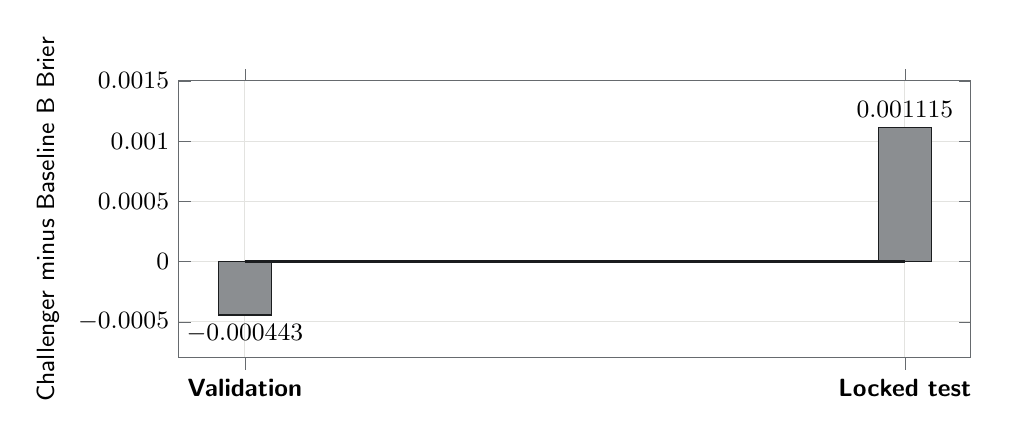
\begin{tikzpicture}
    \begin{axis}[
      width=0.96\textwidth,
      height=51mm,
      ybar,
      bar width=19pt,
      ymin=-0.0008,
      ymax=0.0015,
      symbolic x coords={Validation,Locked test},
      xtick=data,
      ylabel={Challenger minus Baseline B Brier},
      ytick={-0.0005,0,0.0005,0.0010,0.0015},
      scaled y ticks=false,
      y tick label style={font=\small,/pgf/number format/fixed,/pgf/number format/precision=4},
      x tick label style={font=\small\bfseries},
      ylabel style={font=\small},
      axis line style={draw=Muted},
      tick style={draw=Muted},
      grid=major,
      grid style={draw=Pale},
      nodes near coords,
      nodes near coords style={font=\small\bfseries},
      every node near coord/.append style={
        /pgf/number format/fixed,
        /pgf/number format/precision=6
      }
    ]
      \addplot[fill=Mid,draw=Ink] coordinates {
        (Validation,-0.000443388)
        (Locked test,0.001115496)
      };
      \draw[Ink,line width=0.8pt]
        (axis cs:Validation,0) -- (axis cs:Locked test,0);
    \end{axis}
  \end{tikzpicture}
  \caption{The content challenger beat Baseline B slightly on validation, then
  generalized worse on the locked test. Negative is favorable; positive is unfavorable.}
\end{figure}

\vspace{-2mm}
\small
\begin{tabularx}{\textwidth}{@{}L{31mm}Y L{45mm}@{}}
  \toprule
  \textbf{Hypothesis} & \textbf{Evidence} & \textbf{How Phase 2 tests it}\\
  \midrule
  Representation failure &
  The final model selected five train-only adjacency features plus remaining
  duration. Configured semantic features were available but not selected. &
  Replace lexical adjacency with a jointly trained target-prefix encoder and
  discrete hazard head.\\
  Temporal transfer failure &
  Train ended October 9, 2023; validation extended to April 7, 2026; the locked test
  covered April 12 to June 7, 2026. The validation gain did not survive this shift. &
  Use several rolling-origin validation windows and require consistent gains before
  opening a new test.\\
  Target-design failure &
  The largest degradation was on high-frequency targets
  (\(\Delta\) Brier \(=+0.009085\)); phrases were also worse
  (\(+0.001431\)). &
  Audit predictability by target family and redesign targets that are dominated by
  unconditional frequency rather than prefix evidence.\\
  \bottomrule
\end{tabularx}

\vspace{5mm}
\begin{keybox}
  \textbf{Interpretation.}
  The evidence does not justify ``more compute on the same model.'' It justifies an
  experiment that can distinguish the three hypotheses above. Compute becomes useful
  only after the evaluation design can tell us why a model wins or fails.
\end{keybox}

\clearpage

% PAGE 3
\section{Recommended Phase 2 Architecture}

\begin{plainbox}
  \textbf{Primary model: target-conditioned discrete-time neural hazard model}\par
  Given the target, transcript prefix, format, checkpoint, and expected remaining
  length, predict a hazard for the target's first future occurrence in each remaining
  segment. Convert those hazards into the probability of occurrence before the
  transcript ends:
  \[
    P(\text{occurs before end}) =
    1 - \prod_{k=1}^{K}\left(1-h_k\right).
  \]
  Baseline B remains a fixed logit offset. The measured delta therefore answers the
  original question directly: does neural content add information beyond timing and
  target history?
\end{plainbox}

\vspace{4mm}
\begin{center}
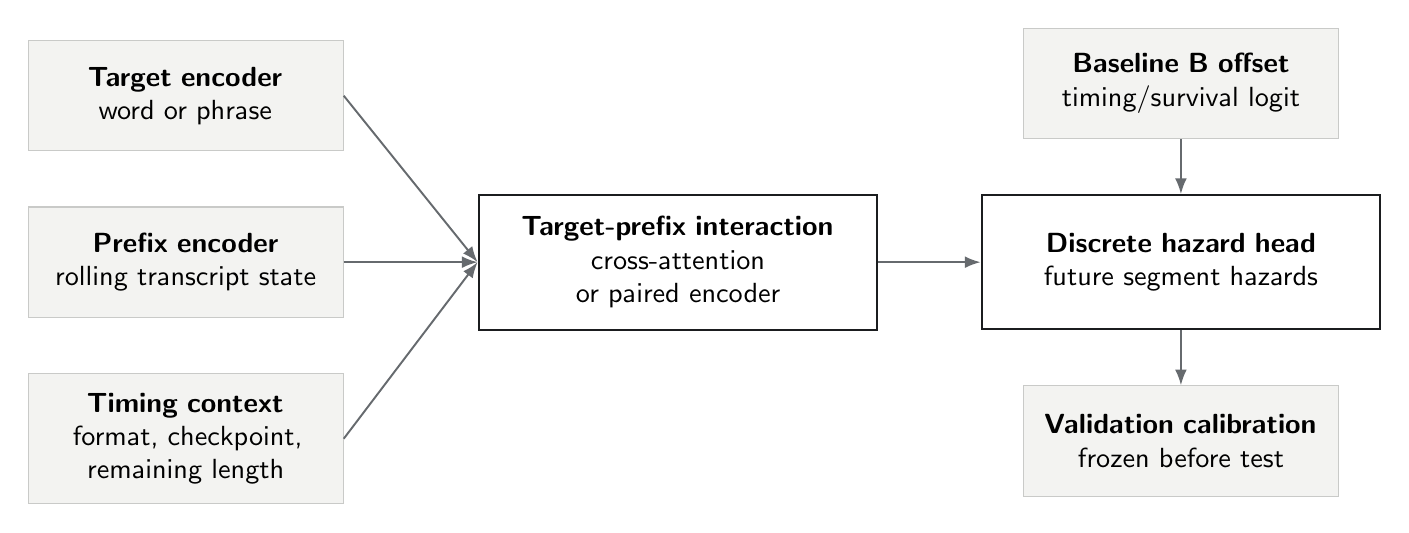
\begin{tikzpicture}[
  node distance=7mm and 7mm,
  box/.style={
    draw=Rule,fill=Soft,minimum height=14mm,text width=35mm,
    align=center,inner sep=2.5mm
  },
  main/.style={
    draw=Ink,fill=white,line width=0.8pt,minimum height=17mm,
    text width=45mm,align=center,inner sep=2.8mm
  },
  arr/.style={-{Latex[length=2mm]},draw=Muted,line width=0.7pt}
]
  \node[box] (target) {\textbf{Target encoder}\\word or phrase};
  \node[box,below=of target] (prefix) {\textbf{Prefix encoder}\\rolling transcript state};
  \node[box,below=of prefix] (meta) {\textbf{Timing context}\\format, checkpoint,\\remaining length};
  \node[main,right=17mm of prefix] (fusion) {\textbf{Target-prefix interaction}\\cross-attention or paired encoder};
  \node[main,right=13mm of fusion] (hazard) {\textbf{Discrete hazard head}\\future segment hazards};
  \node[box,above=of hazard] (offset) {\textbf{Baseline B offset}\\timing/survival logit};
  \node[box,below=of hazard] (cal) {\textbf{Validation calibration}\\frozen before test};

  \draw[arr] (target.east) -- (fusion.west);
  \draw[arr] (prefix.east) -- (fusion.west);
  \draw[arr] (meta.east) -- (fusion.west);
  \draw[arr] (fusion) -- (hazard);
  \draw[arr] (offset) -- (hazard);
  \draw[arr] (hazard) -- (cal);
\end{tikzpicture}
\end{center}

\vspace{3mm}
\small
\begin{tabularx}{\textwidth}{@{}L{38mm}Y L{40mm}@{}}
  \toprule
  \textbf{Candidate} & \textbf{Purpose} & \textbf{Role}\\
  \midrule
  Neural hazard model &
  Learns how target relevance evolves across the remaining transcript while preserving
  explicit time-to-event structure. &
  \textbf{Primary model}\\
  Retrieval-augmented forecaster &
  Retrieves historically similar target-prefix states and uses their observed
  continuations as transparent evidence. &
  Diagnostic / ensemble\\
  LoRA target-conditioned transformer &
  Tests whether parameter-efficient adaptation can learn richer target-prefix
  interactions than a frozen encoder. &
  GPU arm after Gate 1\\
  \bottomrule
\end{tabularx}

\vspace{5mm}
\begin{keybox}
  \textbf{Why this is materially different.}
  The failed system summarized train-era lexical neighborhoods. The proposed system
  learns a shared interaction between an arbitrary target and the evolving transcript
  state, while modeling how opportunity decays as the transcript approaches its end.
\end{keybox}

\clearpage

% PAGE 4
\section{Execution Sequence and Decision Gates}

\begin{enumerate}
  \item \textbf{Gate 0: rebuild the evaluation frontier.}
  Create multiple rolling chronological folds, preserve transcript-level separation,
  and reserve a genuinely new final test period or independent source corpus.

  \item \textbf{Gate 1: prove content signal before expensive tuning.}
  Train a compact target-conditioned encoder and hazard head. Continue only if it
  improves Brier on most rolling folds, on \(t>0\) rows, and against a blank-prefix
  ablation.

  \item \textbf{Gate 2: spend GPU on the strongest hypothesis.}
  Compare frozen encoder, retrieval augmentation, and LoRA under identical folds,
  calibration, target lists, and compute accounting. Select using validation only.

  \item \textbf{Gate 3: freeze and open one new test.}
  Freeze architecture, hyperparameters, calibrator, and decision thresholds. Run all
  arms together once. Report transcript-level bootstrap intervals and contamination-
  pruned results.
\end{enumerate}

\vspace{3mm}
\begin{tabularx}{\textwidth}{@{}L{47mm}L{42mm}Y@{}}
  \toprule
  \textbf{Pre-test continuation gate} & \textbf{Minimum evidence} & \textbf{Why}\\
  \midrule
  Rolling chronological consistency &
  Positive Brier improvement on at least 3 of 4 folds; no large adverse fold &
  Prevents one favorable period from authorizing the test.\\
  After-start usefulness &
  Positive improvement on \(t>0\) rows with transcript-bootstrap support &
  Confirms that live prefix content, not only \(t=0\), carries signal.\\
  Content contribution &
  Full-prefix arm materially beats blank-prefix arm; content share at least 0.5 &
  Demonstrates that transcript content is the source of improvement.\\
  Target-family stability &
  No material regression on high-frequency targets; report phrases and cold targets &
  Addresses the largest failure concentration in the first sprint.\\
  Calibration &
  Challenger ECE no more than 0.01 above Baseline B &
  Keeps probability quality aligned with the original objective.\\
  Operational feasibility &
  Latency, memory, tokens, and dollar cost recorded for a complete pass &
  Prevents an accurate but unusable method from advancing.\\
  \bottomrule
\end{tabularx}

\vspace{5mm}
\begin{keybox}
  {\large\bfseries Final recommendation}\par
  \vspace{1mm}
  Do not reopen or tune against the current locked test. Preserve the completed
  \textbf{STOP} decision. Approve a separate Phase 2 only if its objective is to test
  a genuinely target-conditioned neural representation under rolling time-shift
  validation and a newly sealed evaluation.
\end{keybox}

\vspace{5mm}
\subsection{Research grounding}
The proposed design follows two established principles: dynamic time-to-event
prediction should update risk as longitudinal context changes, and model selection
under real-world distribution shift should evaluate performance across distinct
environments rather than a single random split.

\begin{enumerate}[label={[\arabic*]},leftmargin=7mm,itemsep=1.5pt]
  \item Changhee Lee, Jinsung Yoon, and Mihaela van der Schaar.
  \textit{Dynamic-DeepHit: A Deep Learning Approach for Dynamic Survival Analysis
  With Competing Risks}. AAAI, 2020.
  \href{https://ojs.aaai.org/index.php/AAAI/article/view/5965}{AAAI article}.
  \item Pang Wei Koh et al.
  \textit{WILDS: A Benchmark of in-the-Wild Distribution Shifts}.
  ICML, 2021.
  \href{https://proceedings.mlr.press/v139/koh21a.html}{PMLR article}.
\end{enumerate}

\end{document}
